\lecture_date{Nov 20 2026}
\chapter{Lecture 11}

Using theory developed in the \autoref{subsec:stationary-point-and-classification-1}, we will see an example:
\begin{example}\label{ex:lecture-11-1}
	Consider the quadratic function
	\begin{equation}
		f(\mathbf{x}) = x_1^2 - 2x_2^2 + 3x_3^2 - 4x_1x_2 + 5x_2x_3 - 6x_3x_1 + 7x_1 - 8x_2 + 9x_3 - 10.
		\label{eq:lecture-11-1}
	\end{equation}

	Let
	\[
		\mathbf{x} =
		\begin{bmatrix}
			x_1 \\ x_2 \\ x_3
		\end{bmatrix},
		\qquad
		A_s =
		\begin{bmatrix}
			1  & -2          & -3          \\
			-2 & -2          & \frac{5}{2} \\
			-3 & \frac{5}{2} & 3
		\end{bmatrix},
		\qquad
		\mathbf{b} =
		\begin{bmatrix}
			7 \\ -8 \\ 9
		\end{bmatrix}.
	\]

	Then
	\[
		f(\mathbf{x}) = \mathbf{x}^T A_s \mathbf{x} + \mathbf{b}^T \mathbf{x} - 10.
	\]
	Therefore, stationary point is
	\begin{equation}
		\begin{aligned}
			\mathbf{x}^* & = -\frac{1}{2}A_s^{-1}\mathbf{b} \\
			\mathbf{x}^*
			             & = -\frac{1}{2}\cdot\frac{1}{95}
			\begin{bmatrix}
				-49 & -6  & -44 \\
				-6  & -24 & 14  \\
				-44 & 14  & -24
			\end{bmatrix}
			\begin{bmatrix}
				7 \\ -8 \\ 9
			\end{bmatrix}                                  \\[8pt]
			             & = -\frac{1}{190}
			\begin{bmatrix}
				-691 \\ 276 \\ -636
			\end{bmatrix}                              \\[8pt]
			             & =
			\begin{bmatrix}
				\frac{691}{190} \\[4pt]
				-\frac{138}{95} \\[4pt]
				\frac{318}{95}
			\end{bmatrix}.
		\end{aligned}
		\label{eq:lecture-11-2}
	\end{equation}

	(Using online program) The eigenvalues of $A_s$ are
	\[
		\begin{aligned}
			\lambda_1 & \approx 6.38,  \\
			\lambda_2 & \approx -3.23, \\
			\lambda_3 & \approx -1.15.
		\end{aligned}
	\]

	Since
	\[
		\lambda_1 > 0,
		\qquad
		\lambda_2 < 0,
		\qquad
		\lambda_3 < 0,
	\]
	\( A_s \) is indefinite.

	Therefore,
	\(
	\mathbf{x}^* =
	\begin{bmatrix}
		\frac{691}{190} \\[4pt]
		-\frac{138}{95} \\[4pt]
		\frac{318}{95}
	\end{bmatrix}
	\)
	is a saddle point.
\end{example}

\section{Linear regression}
In this section, we will learn linear regression, the simplest machine learning algorithm. Suppose we have the following graph, where \( x \)-axis represents land area (sq feet) of \( N \) houses and \( y \)-axis represents corresponding house price:

\begin{center}
	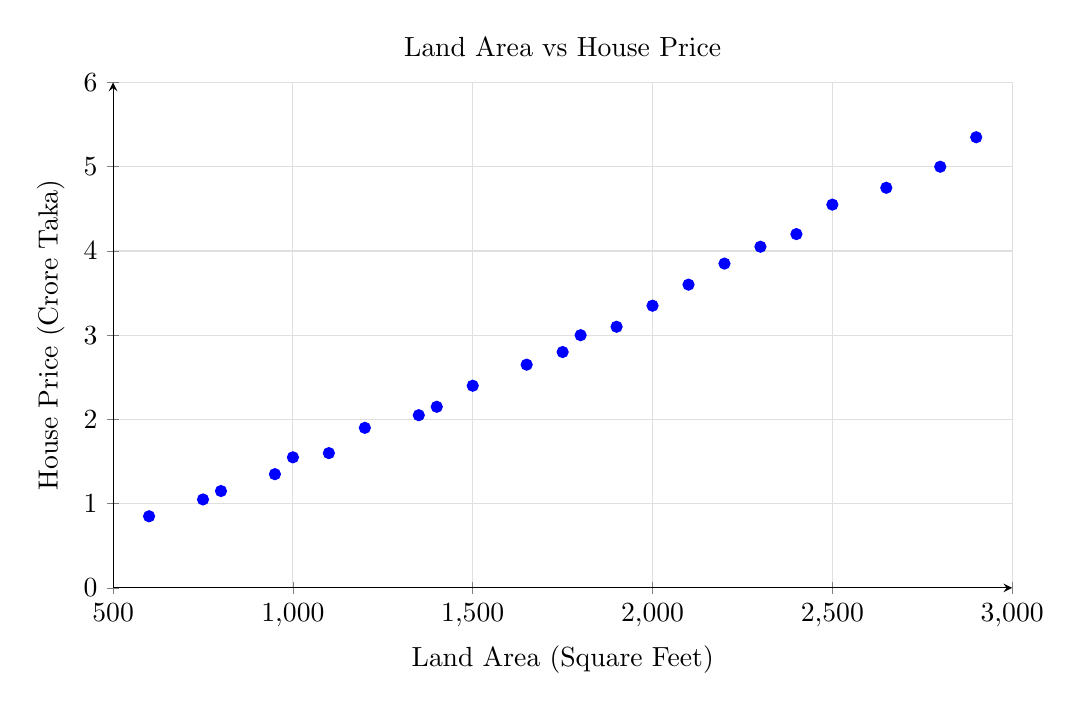
\begin{tikzpicture}
		\begin{axis}[
				width=13cm,
				height=8cm,
				title={Land Area vs House Price},
				xlabel={Land Area (Square Feet)},
				ylabel={House Price (Crore Taka)},
				xmin=500, xmax=3000,
				ymin=0, ymax=6,
				xtick={500,1000,1500,2000,2500,3000},
				ytick={0,1,2,3,4,5,6},
				grid=major,
				grid style={gray!25},
				axis lines=left,
			]
			\addplot[
				only marks,
				mark=*,
				mark size=2pt,
				blue
			] coordinates {
					(600,0.85)
					(750,1.05)
					(800,1.15)
					(950,1.35)
					(1000,1.55)
					(1100,1.60)
					(1200,1.90)
					(1350,2.05)
					(1400,2.15)
					(1500,2.40)
					(1650,2.65)
					(1750,2.80)
					(1800,3.00)
					(1900,3.10)
					(2000,3.35)
					(2100,3.60)
					(2200,3.85)
					(2300,4.05)
					(2400,4.20)
					(2500,4.55)
					(2650,4.75)
					(2800,5.00)
					(2900,5.35)
				};
		\end{axis}
	\end{tikzpicture}
\end{center}

Each point represents a house with land area \(x_k\) and price \(y_k\), where \(k=1,2,\ldots,N\). In machine learning, predicting a numerical value is called a \emph{regression task}, whereas predicting a category is called a \emph{classification task}.

In linear regression, we want to fit a straight line through these data points. The equation of the line is
\[
	\hat{y}=mx+c,
\]
where \(m\) is the slope, \(c\) is the \(y\)-intercept, and \(\hat{y}\) denotes the predicted value (whereas \(y\) denotes the actual value).

Our goal is to find \(m\) and \(c\) such that the line best fits the data. For the \(k\)-th data point, the absolute error is
\[
	e_k=|y_k-\hat{y}_k|=|mx_k+c-y_k|.
\]
We could minimise the average absolute error
\[
	E(m,c)=\frac{1}{N}\sum_{k=1}^{N}|mx_k+c-y_k|.
\]
However, the absolute value function is not differentiable at zero. So we consider the average of the squared errors, called the \emph{mean squared error (MSE)}:
\begin{equation}
	E(m,c)=\frac{1}{N}\sum_{k=1}^{N}(mx_k+c-y_k)^2.
	\label{eq:lecture-11-3}
\end{equation}
Squaring ensures that positive and negative errors do not cancel. We want to minimise this function with respect to \(m\) and \(c\), so we set
\[
	\frac{\partial E}{\partial m}=0,
	\qquad
	\frac{\partial E}{\partial c}=0.
\]
Notice that we are minimizing the error, not necessarily making it zero, since the data points need not lie exactly on a straight line.

Now, the price of a house may depend on several factors besides its land area, such as location, number of rooms, and age. Suppose each data point has \(n\) input variables. Then our dataset consists of \(N\) observations:

\begin{equation*}
	\begin{gathered}
		\bigl(x_1^{(1)},x_2^{(1)},\ldots,x_n^{(1)},y^{(1)}\bigr), \\
		\bigl(x_1^{(2)},x_2^{(2)},\ldots,x_n^{(2)},y^{(2)}\bigr), \\
		\vdots                                        \\
		\bigl(x_1^{(N)},x_2^{(N)},\ldots,x_n^{(N)},y^{(N)}\bigr).
	\end{gathered}
	\label{eq:linear-regression-1}
\end{equation*}
Here, the superscript indicates the data point, not a power, and the subscript indicates the input variable.

The prediction model becomes
\[
	\hat{y}=m_1x_1+m_2x_2+\cdots+m_nx_n+c.
\]
Let
\[
	\mathbf{m}=
	\begin{bmatrix}
		m_1 \\m_2\\\vdots\\m_n
	\end{bmatrix},
	\qquad
	\mathbf{x}=
	\begin{bmatrix}
		x_1 \\x_2\\\vdots\\x_n
	\end{bmatrix}.
\]
Then the prediction can be written as
\[
	\hat{y}=\mathbf{m}^T\mathbf{x}+c.
\]
Therefore, the loss function is
\[
	L(\mathbf{m},c)
	=\frac{1}{N}\sum_{k=1}^{N}
	\left(\mathbf{m}^T\mathbf{x}^{(k)}+c-y^{(k)}\right)^2.
\]
We want to find the weights \(\mathbf{m}\) and intercept \(c\) that minimise this loss.

\subsection{Linear least squares}

We now express the loss function in matrix form. First, consider two data points with one input variable. The vector of prediction errors is
\[
	\begin{bmatrix}
		x^{(1)} & 1 \\
		x^{(2)} & 1
	\end{bmatrix}
	\begin{bmatrix}
		m \\c
	\end{bmatrix}
	-
	\begin{bmatrix}
		y^{(1)} \\y^{(2)}
	\end{bmatrix}
	=
	\begin{bmatrix}
		x^{(1)}m+c-y^{(1)} \\
		x^{(2)}m+c-y^{(2)}
	\end{bmatrix}.
\]
The squared Euclidean norm of this vector is the sum of the squared errors.

For \(N\) data points with \(n\) input variables, define
\[
	X=
	\begin{bmatrix}
		x_1^{(1)} & x_2^{(1)} & \cdots & x_n^{(1)} & 1      \\
		x_1^{(2)} & x_2^{(2)} & \cdots & x_n^{(2)} & 1      \\
		\vdots    & \vdots    & \ddots & \vdots    & \vdots \\
		x_1^{(N)} & x_2^{(N)} & \cdots & x_n^{(N)} & 1
	\end{bmatrix},
	\quad
	\mathbf{w}=
	\begin{bmatrix}
		m_1 \\m_2\\\vdots\\m_n\\c
	\end{bmatrix},
	\quad
	\mathbf{y}=
	\begin{bmatrix}
		y^{(1)} \\y^{(2)}\\\vdots\\y^{(N)}
	\end{bmatrix}.
\]
Here,
\[
	X\in\mathbb{R}^{N\times(n+1)},
	\qquad
	\mathbf{w}\in\mathbb{R}^{n+1},
	\qquad
	\mathbf{y}\in\mathbb{R}^{N}.
\]
The matrix \(X\) contains the input data together with a column of ones to account for the intercept \(c\). The vector \(\mathbf{w}\) contains all the unknown parameters, while \(\mathbf{y}\) contains the actual outputs.

Thus, \(X\mathbf{w}\) is the vector of predictions, and \(X\mathbf{w}-\mathbf{y}\) is the vector of errors. Since the sum of the squares of the components of a vector is its squared Euclidean norm, our loss function becomes
\begin{equation}
	L(\mathbf{w})=\frac{1}{N}\|X\mathbf{w}-\mathbf{y}\|^2.
	\label{eq:lecture-11-4}
\end{equation}

Recall that \(\|\mathbf{u}\|^2=\langle\mathbf{u},\mathbf{u}\rangle=\mathbf{u}^T\mathbf{u}\). Expanding \autoref{eq:lecture-11-4}, we get
\[
	\begin{aligned}
		L(\mathbf{w})
		 & =\frac{1}{N}\langle X\mathbf{w}-\mathbf{y},
		X\mathbf{w}-\mathbf{y}\rangle                  \\
		 & =\frac{1}{N}(X\mathbf{w}-\mathbf{y})^T
		(X\mathbf{w}-\mathbf{y})                       \\
		 & =\frac{1}{N}\left(
		\mathbf{w}^TX^TX\mathbf{w}
		-\mathbf{w}^TX^T\mathbf{y}
		-\mathbf{y}^TX\mathbf{w}
		+\mathbf{y}^T\mathbf{y}
		\right)                                        \\
		 & =\frac{1}{N}\left(
		\mathbf{w}^TX^TX\mathbf{w}
		-2\mathbf{y}^TX\mathbf{w}
		+\mathbf{y}^T\mathbf{y}
		\right),
	\end{aligned}
\]
where we used \((AB)^T=B^TA^T\) and the symmetry of the real inner product.

Notice that \(X\) and \(\mathbf{y}\) are known, while \(\mathbf{w}\) is our variable. Hence, \(L(\mathbf{w})\) is a quadratic function of \(\mathbf{w}\), of the form
\[
	f(\mathbf{x})=\mathbf{x}^TA_s\mathbf{x}
	+\mathbf{b}^T\mathbf{x}+d.
\]
Comparing the two expressions, we obtain
\[
	A_s=\frac{1}{N}X^TX,
	\qquad
	\mathbf{b}=-\frac{2}{N}X^T\mathbf{y},
	\qquad
	d=\frac{1}{N}\mathbf{y}^T\mathbf{y}.
\]
Moreover,
\[
	(X^TX)^T=X^TX,
\]
so \(A_s\) is already symmetric.

Using \autoref{thm:lec10-stationary}, and assuming \(X^TX\) is invertible,
\[
	\begin{aligned}
		\mathbf{w}^*
		 & =-\frac{1}{2}A_s^{-1}\mathbf{b}     \\
		 & =-\frac{1}{2}
		\left(\frac{1}{N}X^TX\right)^{-1}
		\left(-\frac{2}{N}X^T\mathbf{y}\right) \\
		 & =(X^TX)^{-1}X^T\mathbf{y}.
	\end{aligned}
\]
Therefore, the optimal weights are
\begin{equation}
	\boxed{\mathbf{w}^*=(X^TX)^{-1}X^T\mathbf{y}}.
	\label{eq:lecture-11-5}
\end{equation}
This is the \emph{normal equation} for linear least squares.

Since
\[
	\mathbf{v}^TX^TX\mathbf{v}
	=\|X\mathbf{v}\|^2\geq 0
\]
for every \(\mathbf{v}\), the matrix \(X^TX\) is positive semidefinite. If \(X\) has full column rank, then \(X^TX\) is positive definite, and \(\mathbf{w}^*\) is the unique global minimum of the loss function. If \(X^TX\) is singular, the inverse formula does not apply, although least-squares minimisers still exist.

Thus, given a dataset, we construct \(X\) by adding a column of ones to the input data, collect the actual outputs in \(\mathbf{y}\), and use \autoref{eq:lecture-11-5} to obtain the optimal weights.

Although this gives a closed-form solution, computing it can be expensive for large datasets. For example, if \(N=10^6\) and \(n=1000\), then
\[
	X\in\mathbb{R}^{10^6\times1001},
	\qquad
	X^TX\in\mathbb{R}^{1001\times1001}.
\]
Computing \(X^TX\) and its inverse requires substantial computation. Consequently, gradient-based optimization methods are often used instead.

The method is called \emph{linear least squares} because the prediction model is linear in its parameters, and we minimise the mean squared error.

\section{Max function}

Consider the function \(f:\mathbb{R}\to\mathbb{R}\) defined by
\[
	f(x)=\max(x,a),
\]
where \(a\in\mathbb{R}\) is a fixed parameter. Equivalently,
\[
	f(x)=
	\begin{cases}
		a, & x\leq a, \\
		x, & x>a.
	\end{cases}
\]
For example, if \(a=2\), then
\[
	f(x)=\max(x,2)=
	\begin{cases}
		2, & x\leq 2, \\
		x, & x>2.
	\end{cases}
\]

\begin{center}
	\begin{tikzpicture}
		\begin{axis}[
				width=10cm,
				height=6cm,
				axis lines=middle,
				xlabel={$x$},
				ylabel={$f(x)$},
				xmin=-2, xmax=5,
				ymin=-0.5, ymax=5,
				xtick={2},
				ytick={2},
				clip=false,
			]
			\addplot[thick,blue,domain=-2:2] {2};
			\addplot[thick,blue,domain=2:4.7] {x};
			\addplot[only marks,mark=*,blue] coordinates {(2,2)};
			\draw[dashed,red] (axis cs:2,0) -- (axis cs:2,2);
			\node[above left] at (axis cs:2,2) {$(2,2)$};
		\end{axis}
	\end{tikzpicture}
\end{center}

For \(x<2\), the function is constant, so its derivative is zero. For \(x>2\), the function is \(f(x)=x\), so its derivative is one. At \(x=2\), the left-hand derivative is zero and the right-hand derivative is one; hence, the derivative does not exist.

In general,
\[
	f'(x)=
	\begin{cases}
		0, & x<a, \\
		1, & x>a,
	\end{cases}
\]
and \(f'(a)\) does not exist.

A special case is
\[
	\operatorname{ReLU}(x)=\max(x,0)
	=
	\begin{cases}
		0, & x\leq 0, \\
		x, & x>0.
	\end{cases}
\]
This is called the \emph{Rectified Linear Unit (ReLU)} activation function, commonly used in machine learning.

When applying the chain rule in automatic differentiation (forward or reverse mode), we need a derivative value for each operation. Although the max function is not differentiable at \(x=a\), a convention is adopted at that point. In this course, we use
\[
	Df(x)=
	\begin{cases}
		0, & x\leq a, \\
		1, & x>a,
	\end{cases}
\]
where \(Df(a)=0\) is an assigned value, not the ordinary derivative. Other implementations may assign \(1\) at \(x=a\). Away from that point, \(Df(x)=f'(x)\).

For ReLU, this gives
\[
	D\operatorname{ReLU}(x)=
	\begin{cases}
		0, & x\leq 0, \\
		1, & x>0.
	\end{cases}
\]
This convention allows us to use the max function in automatic differentiation.
